Desde el punto de vista de la biología computacional el cáncer puede ser visto como un sistema ecológico y de comportamiento emergente.
Lo cual, hace apropiado el uso de autómatas celulares para simular su comportamiento. Es por ello que, cada vez más se opta por el uso
de simulaciones por ordenador como la que se presenta en este trabajo ayudando, desde el estudio y comprensión del cáncer, hasta
el estudio y desarrollo de nuevas terapias contra él.

El cáncer es una enfermedad cada vez más común debido a sus muy diversos factores que propician su aparición, esto es,
mayor esperanza de vida de la población y, por tanto, individuos cuyas células han sufrido más mutaciones, factores ambientales y/o
formas de vida poco saludables, mayor estrés de la población, y hasta exposición a fuentes de radiación artificiales.

A pesar de todo, el cuerpo tiene una serie de mecanismos para prevenir la aparición y la proliferación de esta enfermedad. Estos,
son muchos y muy diversos, así como, los mecanismos propios de las células que intervienen en este proceso. En esta simulación, por tanto,
se pretende tener en cuenta el enfoque de los autores del trabajo original, eligiendo sólo un subconjunto de todas estas
características y comportamientos.

La elección de un autómata celular como enfoque para modelizar el comportamiento de esta enfermedad proviene por la relativa
facilidad de obtener comportamientos complejos a partir de una reglas relativamente sencillas a nivel local en cada célula.

Este trabajo, como se ha comentado previamente, pretende reproducir el trabajo de José Santos y Ángel Monteagudo \cite{jsantos-amonteagudo-1-2014},
uno de los trabajos \cite{jsantos-amonteagudo-2012} \cite{jsantos-amonteagudo-2013} \cite{jsantos-amonteagudo-2015} que dichos autores han realizado siguiendo la idea de realizar simulaciones sobre esta enfermedad y, por ello, aquí
se realiza una nueva implementación con el fin de reproducir los resultados obtenidos en el citado artículo.

\newpage

La implementación consiste en seguir un modelo de eventos, es decir, se pretende simular el proceso que siguen las células para su división, que
consiste en, la realización de una serie de pruebas para comprobar si la célula debe reproducirse, la realización de la propia división, y
la programación de un nuevo evento de división en el futuro. A lo largo de la ejecución del programa en cada iteración puede haber ninguna, una o
varias células que deben seguir el proceso que se acaba de describir brevemente.

Finalmente, para estudiar el comportamiento del cáncer se realizan diversas ejecuciones utilizando diferentes parámetros y configuraciones,
y observando en cada caso qué factor es el que provoca el cambio en el comportamiento global.

\section{Objetivos}

En este trabajo, se esperan alcanzar los siguientes objetivos:

\begin{itemize}
  \item Encontrar artículos científicos de calidad sobre esta temática.
  \item Extraer información del artículo (o los artículos).
  \item Elegir un artículo y hacer una implementación propia.
  \item Reproducir los resultados del artículo.
  \item Comparar los resultados obtenidos con los del artículo.
\end{itemize}

\section{Alcance}

El presente trabajo tiene como finalidad reproducir el trabajo de José Santos y Ángel Monteagudo \cite{jsantos-amonteagudo-1-2014}, realizando
una implementación propia del sistema que se describe en su artículo.

No obstante, el comportamiento que se pretende simular cuenta con una serie de pasos en los cuales el comportamiento dependerá
de ciertos sorteos con una probabilidad dada. Esta es una limitación a tener en cuenta a la hora de obtener los mismos resultados
que los autores de dicho trabajo.

\section{El cáncer}

El cáncer es el nombre genérico usado para referirse a más de $200$ enfermedades cuyo resultado
es la proliferación descontrolada de las células que se ven afectadas. Aunque no era común
encontrar signos de cáncer en los seres vivos en la antigüedad debido a una menor esperanza
media de vida, lo cierto es que es inherente al reino animal.

El origen etimológico del nombre proviene de la antigua grecia, donde
Hipócrates utilizó los términos \textit{carcino} y \textit{carcinoma} para referirse
a dicha enfermedad, las cuales hacían referencia al cangrejo debido a la forma en la
que se proyectaban los cánceres.

El cáncer se clasifica como:

\begin{itemize}
    \item Una \textbf{enfermedad genética}, debido a, que es causada por un cambio en el
    material genético (\textit{ADN}) de las células.
    \item Una \textbf{enfermedad multigénica}, ya que, afecta a diferentes genes.
    \item Una \textbf{enfermedad multifactorial}, es decir, tiene causas muy diversas.
    \item Una \textbf{enfermedad multiorgánica}, por tanto, afecta a diferentes tejidos y órganos.
\end{itemize}

Se conoce como neoplasia a toda masa anormal que tenga lugar en el cuerpo. Esto es, la división
descontrolada de la célula y el aumento de tamaño de cada una de ellas, y ocurre
por un problema en el \textit{ADN} de la célula, la cual, contiene la información acerca de cuales son
las funciones de la misma.

Al producirse en todo tipo de tejidos la evolución y el tratamiento de esta enfermedad varía.
El factor determinante entre que este tipo de masas anormales sea benigna (adenoma)
o maligna (carcinoma) es el factor de crecimiento y la invasividad de tejido adyacente.

Presenta diferentes fases, partiendo de un crecimiento anormal en tamaño, en la cual,
las células del interior necesitarán más sangre para obtener nutrientes y, en consecuencia,
mueren por necrosis. El tumor puede pasar a una nueva fase, conocida como \textit{angiogénesis},
si adquiere la capacidad de crear nuevos vasos sanguíneos para alimentar a las células
del interior. Esto lo consigue mediante el envío de señales químicas que motiva la creación
de nuevos capilares hacia dentro del tumor.

Finalmente, la célula se vasculariza, es decir, partes de ella pasan
a la sangre, continuando con este comportamiento allí donde se depositen y, además, en muchas
ocasiones se observa metástasis.

Es obvio, que la célula para llegar a la última fase va a necesitar cierto grado de daño genético,
así como, superar determinadas barreras. Por un lado, obtener todas las capacidades necesarias para
poder dividirse sin control, crear sus propios vasos sanguíneos, etc. dependerá de la obtención
de mutaciones en su \textit{ADN} que permita todo esto. Por otro lado, el cuerpo tiene mecanismos para evitar
que esto ocurra, como por ejemplo, muerte por daño genético, evitar enviar orden de división e, incluso,
el propio sistema inmune interviene para intentar evitar su crecimiento, además de otros muchos mecanismos.

Por tanto, esta es una enfermedad compleja de tipo ecológico y emergente, lo cual, dificulta su estudio,
así como, su tratamiento.

\section{Los autómatas celulares}

El patrón mostrado en ciertas conchas marinas, como se muestra en la figura~\ref{fig:conus},
es generado mediante autómatas celulares naturales. Estas conchas muestran un aspecto exterior
en el cual se observan patrones, los cuales les han
permitido en muchas ocasiones ocultarse mejor en su entorno y, por ello, aumentar su supervivencia.
Dichos patrones son de muy diversos tipos, por ejemplo, forman formas reconocibles, o formas fractales,
entre otras.

\begin{figure}[h]
\centering
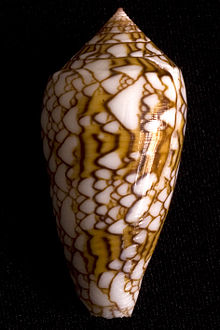
\includegraphics[scale=2]{figures/Conustextile}
\caption{\textit{Conus textile shell}, especie de gasterópodo que presenta un autómata celular natural en su concha.}
\label{fig:conus}
\end{figure}

\newpage

En ellos, cada célula toma un color o forma diferente según sus células vecinas, obedeciendo
a una versión natural de unas reglas matemáticas. Basándose en esto, se conoce como autómata celular
al modelo matemático abstracto que modela sistemas dinámicos que evolucionan en pasos discretos.

Son muy adecuados para ser implementados por ordenadores, útiles para simular comportamientos de sistemas
complejos, como por ejemplo: colonias, epidemias, dinámica de fluidos, etc., y en muy diversas áreas, como por ejemplo,
en física, biología, química, socioeconomía, etc.

En el libro \textit{Simulating Complex Systems by Cellular Automata} de Jiri Kroc, Peter M.A. Sloot y Alfons G. Hoekstra
\cite{cellular-automata} se presentan los fundamentos matemáticos que siguen los autómatas celulares.

Fueron descubiertos por John von Neumann en la década de 1950, aunque basado en trabajos teóricos previos de la
década de 1940. A modo de resumen, los autómatas celulares cuentan con los siguientes componentes:

\begin{itemize}
    \item Red regular de nodos, de cantidad finita o infinita, que representa la estructura espacial.
    \item En cada nodo, se coloca un autómata finito, es decir, representa un número finito de estados posibles.
    Aquellos que se encuentran ocupados, reciben el nombre de células o celdas.
    \item Cada célula se comunica con su entorno, pero sólo con una parte de él. Esto se conoce como vecindario,
    y existen varios tipos, por ejemplo, el vecindario de Moore, o el vecindario de vonNeumann,
    como se muestra en la figura~\ref{fig:neighboor}.
    \item Función que determina la evolución de los estados de las distintas células.
\end{itemize}

\begin{figure}[h]
\centering
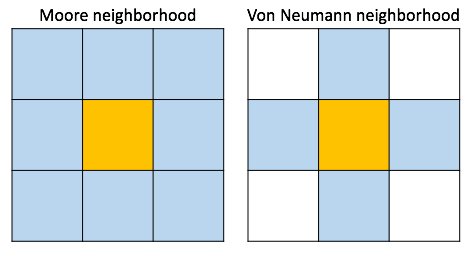
\includegraphics[scale=0.6]{figures/automata_neighboor}
\caption{Tipos de vecindarios en los autómatas celulares.}
\label{fig:neighboor}
\end{figure}

Dada una configuración se puede estudiar las transformaciones aplicando las reglas,
lo que se conoce como órbita. Dichas órbitas pueden ser muy complejas, a pesar de
la sencillez del autómata celular.

Uno de los autómatas celulares más famosos es el \textit{Juego de la vida de Conway}.
Diseñado por el matemático John Horton Conway en la década de $1970$. Es tan famoso debido a
que es equivalente a una máquina universal de Turing o, lo que es lo mismo, es un modelo de computación universal\footnote{\url{http://eprints.uwe.ac.uk/22323/1/thesis.pdf}}.
Esto es, todo lo que se puede computar algorítmicamente se puede computar en el juego de la vida.

Existen, además, muy diversas implementaciones y aplicaciones, como por ejemplo, para hacer música.
En el libro \textit{Game of Life Cellular Automata} de Andrew Adamatzky \cite{game-of-life} se presenta
el juego de la vida, y en el último capítulo se expone una forma de hacer música con él. Para ello, el autor
utiliza cada celda ocupada por un autómata en cada iteración para tocar tres notas utilizando
las coordenadas $(x,y)$ de la posición del autómata en el plano cartesiano. De este modo,
obtiene las tres notas utilizando una nota fija, y dos notas más mediante el valor de
$x$ e $y$ como intervalo entre notas de un piano respecto de la nota fija y de la segunda nota
respectivamente.

Se puede concluir que un autómata celular es una de las formas más adecuadas de simular comportamientos
emergentes y, por tanto, adecuado para este tipo de problemas. José Santos y
Ángel Monteagudo \cite{jsantos-amonteagudo-1-2014} optaron por utilizar autómatas celulares para sus trabajos.

En este caso, los autores pretenden simular el comportamiento emergente que presentan los
tumores mediante un autómata celular. Ellos parten de los trabajos previos de Douglas Hanahan y Robert A. Weinberg
llamados \textit{The hallmarks of cancer} \cite{hanahan-weinberg-2000} y \textit{The hallmarks of cancer: The next generation} \cite{hanahan-weinberg-2011}
respectivamente. En ellos, se identifican una serie de marcadores asociados a ciertas mutaciones presentes
en el genoma de las células que permiten la aparición y evolución de tumores.
